% =============================================================================
% 5.3 混合检索权重扫描与边界分析
% 草稿版本：v0.2 (2026-05-07)
%   v0.1：作为 5.2.2 子小节起草。
%   v0.2：按导师意见 3 提级为 5.3 \subsection；标题去掉前缀"通路 A"
%        以避免清单式命名（意见 7），正文叙述里仍保留"通路 A 混合检索"。
% 字数：约 1300 字
% 风格规则：v0.2 风格（无 \textbf / \textit / 引例括号 / 双引号 / 破折号）
% 引用：\cite{ref12, ref24}
% 图表：
%   - 表 \reftab{tab:rag-mode-comparison}    3 档检索器消融
%   - 图 \reffig{fig:rag-weight-sweep}       8 个权重点 Top-1 / MRR 双 y 轴折线图
%   - 表 \reftab{tab:rag-weight-drift}       最优权重随 KB 体量漂移
% 复用 4.1 节已有图表：\reftab{tab:rag-weight-sweep}（权重扫描总表）
% 依赖宏包：booktabs / tabularx / graphicx（主稿已加载）
% =============================================================================

\subsection{混合检索权重扫描与边界分析}
\label{sec:rag-eval}

通路 A 混合检索的设计原理与权重扫描总表已在 \ref{sec:semantic-bridge}
节给出，本节聚焦三件 \ref{sec:semantic-bridge} 节未展开的内容：3 档
检索器的全维度对照、最优权重随知识库体量动态漂移的工程含义、以及
剩余 9 条 Top-1 脱靶用例的失败模式分类。

评测集为 \texttt{rag\_\bk{}retrieval\_\bk{}bench.\bk{}jsonl} 共 60 条用例，覆盖 8 类
查询场景：概念性查询 \texttt{term}、降水阈值 \texttt{grade\_\bk{}precip}、
蒲福风级 \texttt{grade\_\bk{}wind}、温度分级 \texttt{grade\_\bk{}temp}、能见度
分级 \texttt{grade\_\bk{}visibility}、湿度分级 \texttt{grade\_\bk{}humidity}、
作业适宜性 \texttt{op\_\bk{}*}、跨文档复合 \texttt{multi} 与同义改写
\texttt{paraphrase}。每条用例标注 \texttt{relevant\_\bk{}ids} 金标准 ID
与 \texttt{expected\_\bk{}categories} 类别白名单，用于计算 Top-$K$ 命中率、
MRR、Recall@$K$ 与 Category@$K$ 等指标 \cite{ref24}。MRR 是其中最
关键的指标，因为大语言模型在 RAG 流程中通常仅把 Top-1 与 Top-3 当作
强证据，相关条目的排名分布直接决定下游回答质量 \cite{ref12}。

3 档检索器消融的全维度对照见 \reftab{tab:rag-mode-comparison}。在 60 条
评测集上，纯向量与纯 BM25 的 Top-1 命中率意外打平在 81.7\%。混合检索
\texttt{hybrid (0.9/\bk{}0.1)} 在 Top-1、MRR、Recall@1、Recall@3、Recall@5
五项核心指标上全面胜出，仅 Category@1 略低于纯向量。Recall@5 已经
接近 97.7\% 的天花板水平，意味着 60 条用例中有 58 条的金标准条目
都进入了 Top-5 上下文窗口，剩余 2 条结构性失败构成本节后续分析的
重点。

\begin{table}[H]
    \centering
    \caption{通路 A 三档检索器全维度对照（60 条评测集）}
    \label{tab:rag-mode-comparison}
    \song\fontsize{9pt}{12pt}\selectfont
    \renewcommand{\arraystretch}{0.95}
    \begin{tabular}{lccc}
        \toprule
        指标 & vector & bm25 & hybrid (0.9/0.1) \\
        \midrule
        Top-1 命中率 & 81.7\% & 81.7\% & 85.0\% \\
        MRR & 0.872 & 0.872 & 0.908 \\
        Recall@1 & 73.3\% & 73.3\% & 76.7\% \\
        Recall@3 & 90.0\% & 86.7\% & 91.7\% \\
        Recall@5 & 96.7\% & 91.7\% & 97.7\% \\
        Precision@1 & 81.7\% & 81.7\% & 85.0\% \\
        Category@1 & 96.7\% & 88.3\% & 95.0\% \\
        Top-1 脱靶用例数 & 11 & 11 & 9 \\
        \bottomrule
    \end{tabular}
\end{table}

混合检索的边际增益是真实存在的，且向量检索与 BM25 在错误样本上是
互补的。纯向量在概念性查询上稳定，纯 BM25 在阈值数字类查询上稳定，
两类强项正交。这一互补性是混合可以同时优于二者 3.3 个百分点的工程
前提。\reftab{tab:rag-weight-sweep} 在 \ref{sec:semantic-bridge} 节
给出了 8 个权重点的完整扫描结果，对应的可视化走势见
\reffig{fig:rag-weight-sweep}：当 $\alpha$ 从 0.50 上升至 0.90 时
Top-1 命中率与 MRR 同步抬升至 85.0\% 与 0.908 双双触顶，随后在 1.00
回落，证实存在唯一最优工作点而非单调走势。

\begin{figure}[!ht]
    \centering
    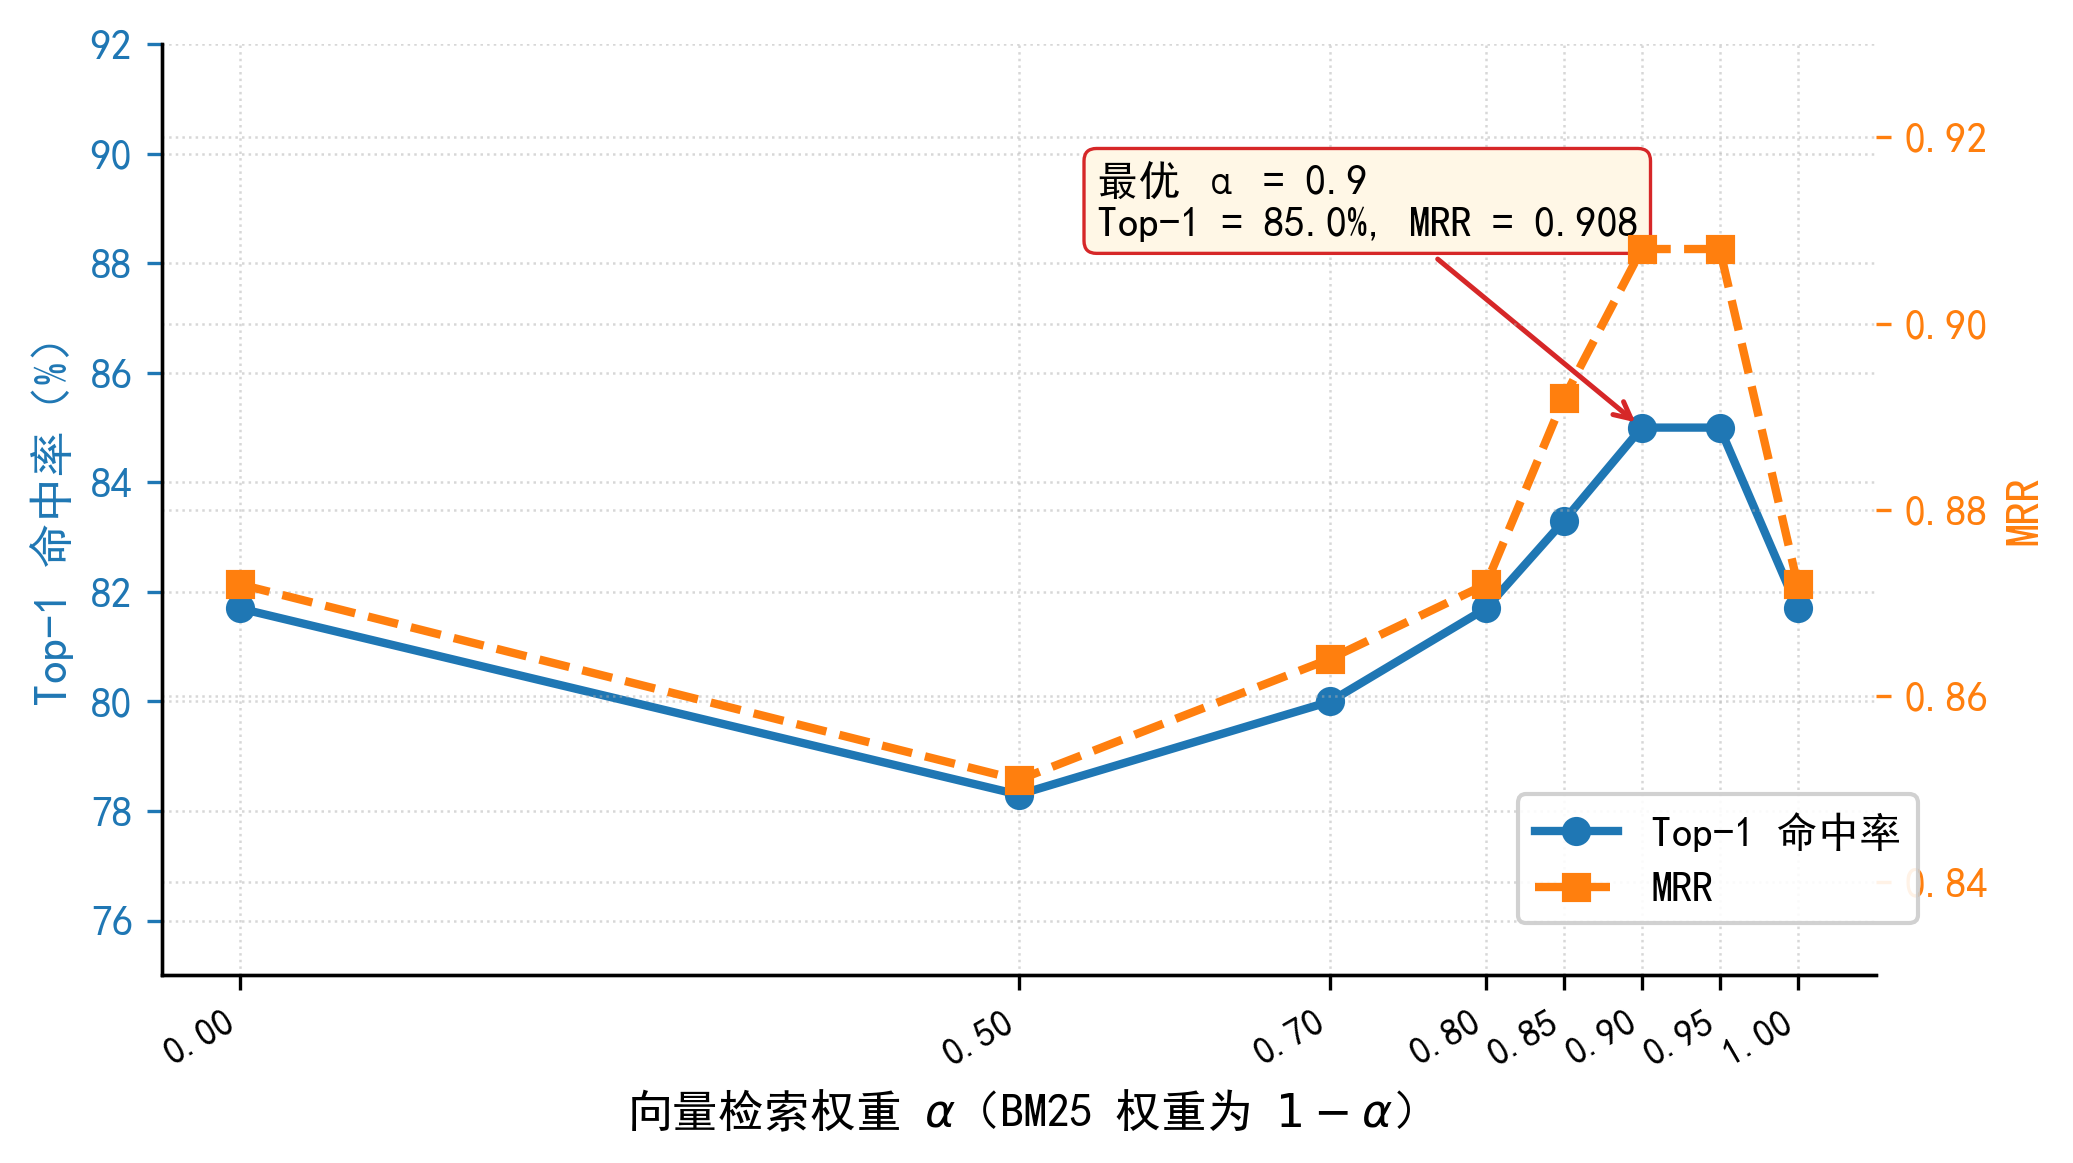
\includegraphics[width=0.85\linewidth]{figures/eval_5_1_rag_weight_sweep}
    \caption{通路 A 混合检索权重扫描走势（60 条评测集，左轴 Top-1 命中率，右轴 MRR）}
    \label{fig:rag-weight-sweep}
\end{figure}

本节进一步对照两轮不同知识库体量下的最优权重，结果见
\reftab{tab:rag-weight-drift}。

\begin{table}[H]
    \centering
    \caption{最优混合检索权重随知识库体量的动态漂移}
    \label{tab:rag-weight-drift}
    \song\wuhao
    \begin{tabular}{lcccc}
        \toprule
        知识库版本 & 知识条目数 & 评测集规模 & 最优 $\alpha$ & 最优 Top-1 \\
        \midrule
        v1.0 (precip + wind) & 44 & 43 & 0.80 & 90.7\% \\
        v1.2 (扩展 temp + vis + humidity) & 62 & 60 & 0.90 & 85.0\% \\
        \bottomrule
    \end{tabular}
\end{table}

最优 $\alpha$ 从 0.80 上调到 0.90 是一条值得在工程实践中借鉴的方法
论结论。知识库扩展后相邻条目语义距离变近，例如温度类的凉、舒适、
温暖三档在向量空间中本就邻近，BM25 在小权重下对相邻词字面匹配反而
成为干扰。即使在 v1.2 版本下，纯向量与纯 BM25 的 Top-1 仍只有
81.7\%，证明 BM25 在少量但关键样本上仍贡献 3.3 个百分点边际增益，
不能去除。混合检索的权重不能一次调好用到底，应随知识库规模重新校准。

剩余的 9 条 Top-1 脱靶用例是论证通路 B 必要性的关键证据。按失败原因
归类，这 9 条可以分为三组。第一组是邻近阈值边界，例如 query 降水
200 毫米算什么级别，正确答案是 GB/T 28592-2012 中大暴雨档
$100\sim249.9\,\mathrm{mm}$，但 200 毫米在向量空间中距离大暴雨与
特大暴雨两条目几乎等距，hybrid 检索器把特大暴雨 $\geq 250\,\mathrm{mm}$
排到了第一。这一类共 5 条，本质是嵌入模型在小型知识库上无法精确
区分相邻阈值的离散归属。第二组是术语别名冲突，例如 query 强风是几级
风，应命中蒲福 6 级专名条目，但强风同时是台风条目高频词，BM25 偏向
出现频次更高的台风条目，向量召回也未能消除这一干扰，共 2 条。第三组
是跨类别多文档召回边界，例如 query 暴雨怎么应对应当跨 grading 与
operation 两个类别召回，但 hybrid 把 \texttt{term\_\bk{}thunderstorm} 排到
首位，共 2 条。

这 9 条失败用例的共性是：靠任何嵌入模型加 BM25 在小型知识库上都难以
精确区分相邻阈值条目。混合检索的工程上限在 85\% 左右，难以单纯靠
权重调整突破。这正是通路 B 即确定性 if-else 分级器加 grade\_id 硬链接
设计的工程必要性。前 7 条邻近阈值与术语别名失败用例在通路 B 上都能
达到 100\% 准确率，构成通路 A 加通路 B 双覆盖闭环的具体实证支撑。
